\documentclass{article}

\usepackage{amsmath}
\usepackage{graphicx}
\usepackage{xcolor}
\usepackage[export]{adjustbox}
\RequirePackage[margin=1in]{geometry}

\newcommand\todo[1]{\textcolor{red}{TODO: #1}}

\newcommand\animation[1]{\textcolor{blue}{ANIMATION: #1}}

\begin{document}
	
\title{Hillshade Video Script}
\author{Nathan Stouffer}
\date{}
\maketitle

\section{Intro}

\subsection{Motivation}

What I'm showing you right now is a map.
But you probably didn't need to be told that.
In fact, I would be willing to bet that you know a lot more than that.
You can probably see that this particular spot is relatively flat and that this other area is pretty steep, that this is a small gully and this is a ridgeline, and that this face is pretty rugged while this slope is not quite as technical.

You are able to get all that complex information from a pretty simple grayscale image.
In fact, I would be willing to bet that your understanding of this map is better than if I had given you the contour lines even though that is a more precise way to convey information.

\animation{Bring in more maps (one with just contours and another with contours/hillshade)}

Here is a side-by-side to compare.
Contours are really useful but they often take a bit more thought to interpret.

This map is intentionally set up so that your brain can intuit the shape of the terrain.
Modern computers do much of this work today, but cartographers have been using versions of this technique for hundreds of years.
And many other applications use similar strategies to help convey geometric information to your brain.

The topic I'd like to discuss today is a lighting technique called hillshade.
We're going to talk about why it's such an effective method of terrain lighting and walk through the math that powers it.

\begin{center}
	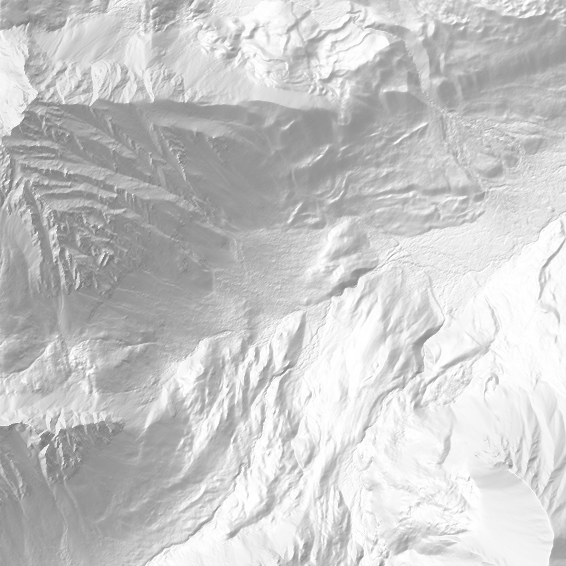
\includegraphics[width=0.5\textwidth,frame]{assets/hillshade-example.png}
\end{center}

\subsection{Directional Lighting}

We'll be discussing hillshade, but it's worth mentioning that hillshade is a very specific example of something called a directional light.
Directional lights are used all over computer graphics and are themselves just one option for how you might want to light a scene.
What I find so intriguing about directional lights is that they give you a lot of bang for your buck.
They give you quite a bit of realism for the amount of effort that you need to expend.

\animation{Fade in a graph similar to the below image.}

\begin{center}
	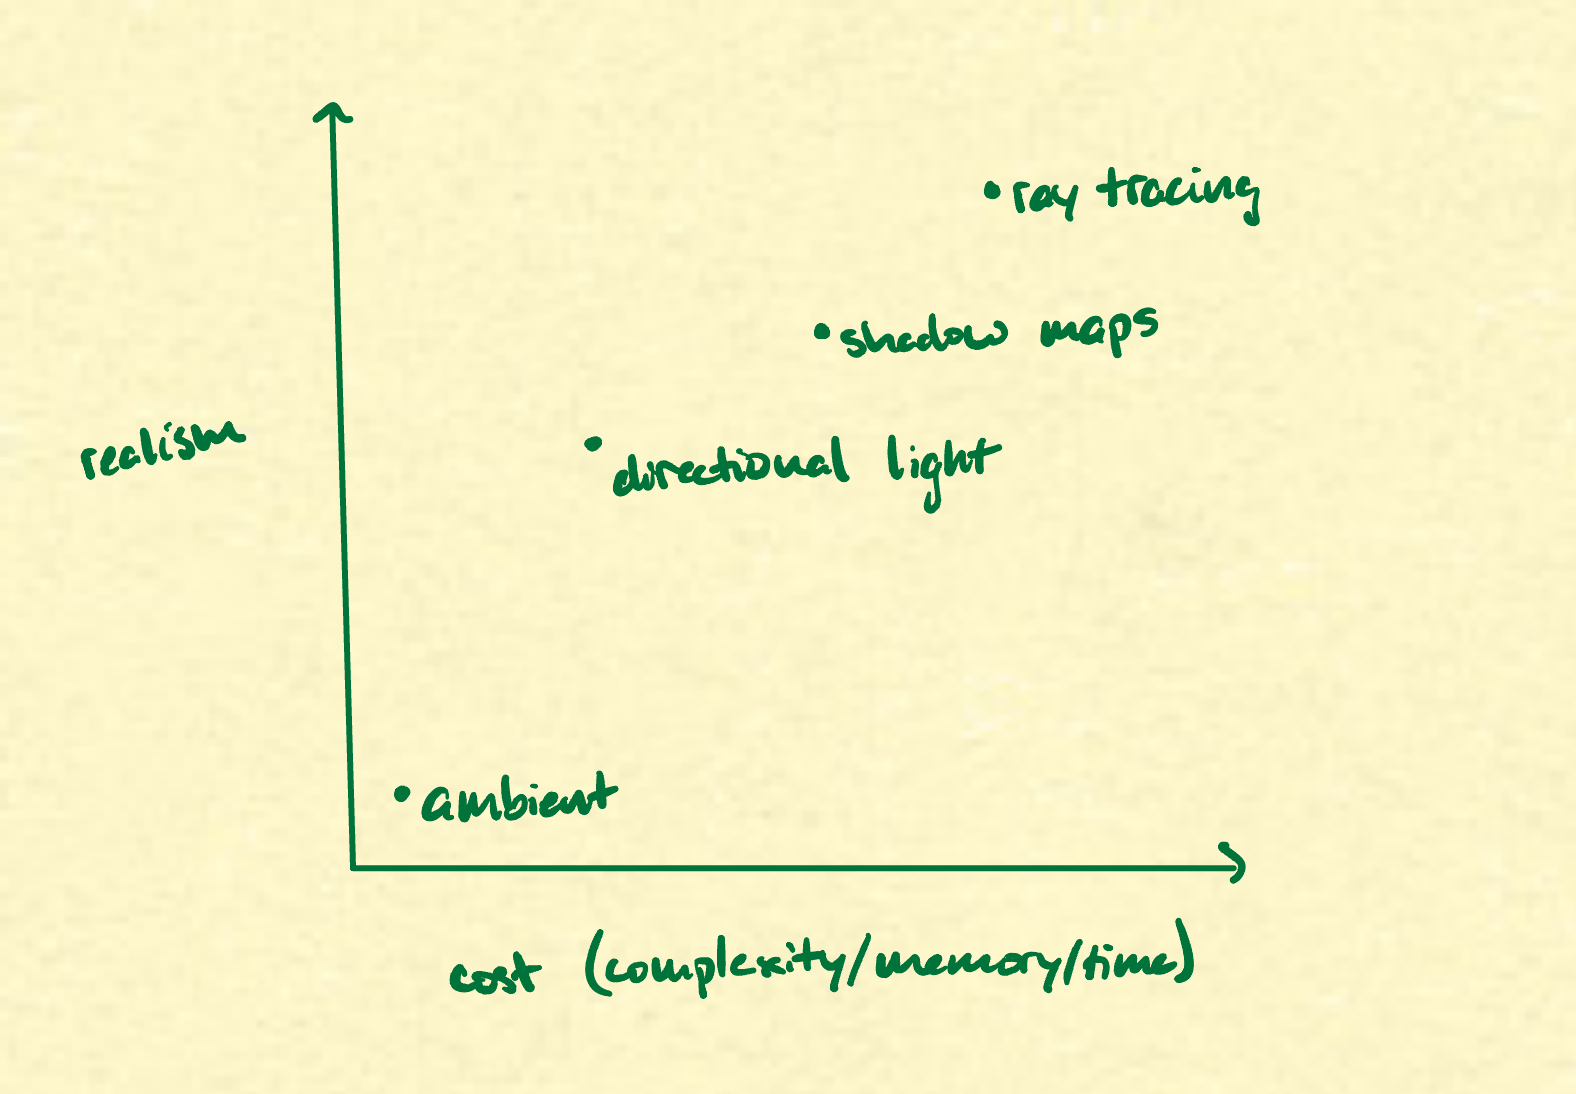
\includegraphics[width=0.65\textwidth,frame]{assets/realism.jpg}
\end{center}

If you were to represent different lighting techniques as points in the plane where the y-axis represents some notion of realism and the x-axis represents some notion of cost (maybe in terms of complexity/memory/computation time).
Then on that graph, directional lights would exist at a sweet spot where they are unreasonably effective.

So what is a directional light?
Well, a directional light is a pseudo-realistic model of how light behaves that takes a few shortcuts in the interest of simplicity.
The shortcuts come in the form of the following assumptions:

\begin{enumerate}
	
\item First, we assume that the light source is extremely far away, essentially infinitely far away.
If that is the case, every point in your scene has light coming from the same direction -- giving the technique gets its name.
Given this direction, you can imagine a directional light as an effect where we light up areas that face the light and leave areas that don't face the light in shadow.

\item The second assumption that is typically made when working with directional lights is that we ignore obstructions.
What this means is that we aren't computing true shadows in the scene -- just whether or not a particular region \textit{faces} the light.
The direction is all that matters.

\end{enumerate}

In our context, the ``direction'' that the terrain faces is encoded in something called a surface normal.
The surface normal at a particular point is a vector that is perpendicular (or more precisely, orthogonal) to the face of the terrain at that point.
The light direction is given to us by configuration.

Though, to make the math a little simpler, I am going to use the negative of the light direction.
This is the vector $l$ that points directly \textit{towards} the light source.

\animation{Show a rotating plane with a surface normal that is lit according to hillshade.}

When zoomed in on a small region of the terrain with surface normal $n$, the effect we are looking for should behave like this:
If $n$ points in the same direction as $l$, we light that region at full strength.
If $n$ is set up so that $l$ kind of glances off the terrain, we light that region at medium strength.
And if $n$ points directly opposite to $l$, we light that region at no strength.

Performing this operation at every pixel in our image results in a lot texture that your brain can intuit to figure out what the terrain looks like in 3-dimensions.

\section{Hillshading}

At this point, we've covered what the effect should do, but how can we accomplish it?
What are the nuts and bolts that take this effect from a discussion of a loosely defined goal to the sequence of mathematical operations that achieve it?

\subsection{Cosine}

We can start by describing exactly how the light strength should vary.
To reason our way through this, it helps to think of what happens to our plane as $n$ rotates away from $l$.
If we assume the light hits the plane evenly, then when the surface normal is aligned with $l$, the light is at full strength $S$.
Then if we watch from the side as we rotate the plane by some angle $\theta$, we can compute the percentage of the original amount of light that hit this plane.
This falls out from the definition of cosine: it is $\cos \theta$.
When $\theta > \pi/2$, the plane is facing away from the light and $\cos \theta < 0$.
Many applications clamp the cosine to $[0, 1]$ because our light strength should always be positive.

\begin{center}
	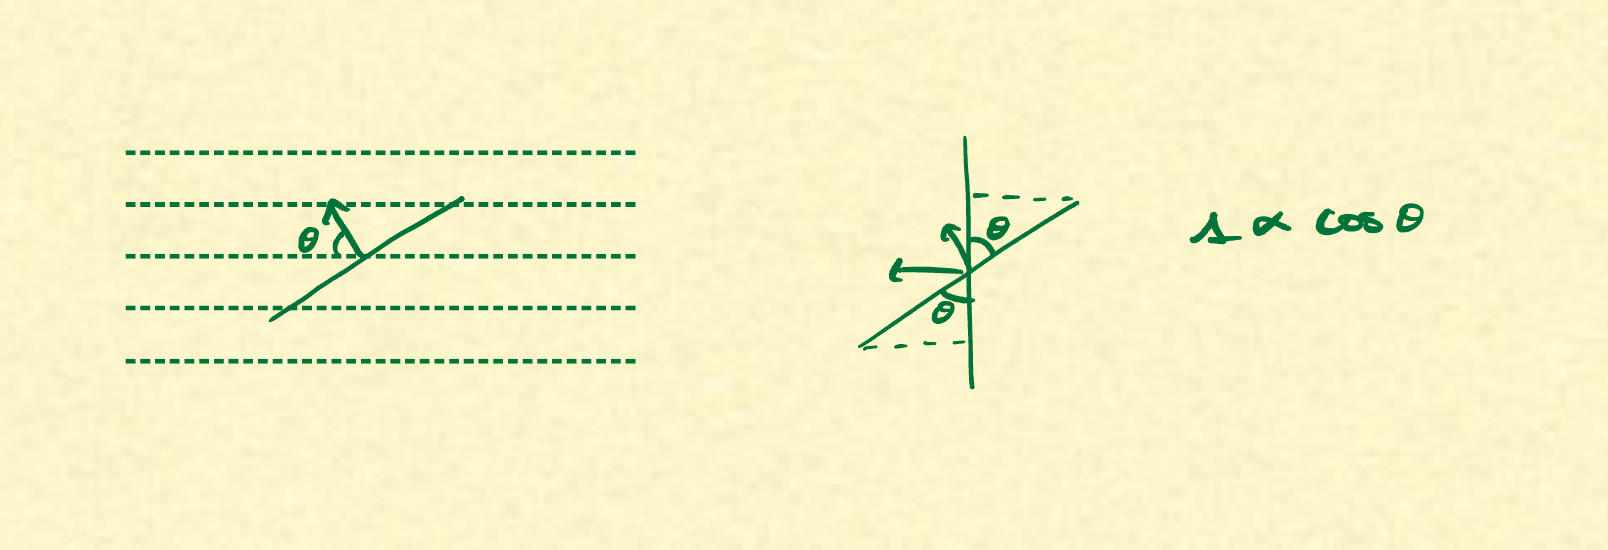
\includegraphics[width=0.75\textwidth,frame]{assets/cosine.jpg}
\end{center}

That derivation works as-is for some contexts, but hillshade usually makes one tweak to that process.
Remember, we want effectively light a map so that the map-reader can see the terrain features.
When we clamp the light strength to the range $[0, 1]$, we effectively remove shading on all terrain that faces away from the light source.
Instead of clamping, it is usually more effective to remap the range of cosine to the interval $[0, 1]$.
This can be done by $\dfrac{1 + \cos \theta}{2}$.

\subsection{Law of Cosines $=>$ Dot Product}

We now know that we want to vary the strength of our lighting according to $\cos \theta$.
But that doesn't really help us much because we don't know what $\theta$ is.
All we know are the vectors $l$ and $n$.
At the end of the day, those are just lists of numbers.
Sure, they have some constraints (like the fact that their length is 1).
And they also have some geometric meaning (they are directions in 3d space).
But when it comes down to it, we need to turn two lists of numbers into something as complex as the cosine function.
How are we supposed to do it?
What is the link between these two vectors and cosine?

If you were some early mathematician, at this point, you would have to start experimenting with ideas and wait for inspiration to strike.
This sort of thing takes practice and often has lots of dead ends.
It's one of those things where experience is the best teacher.

... But if I were to offer one piece of advice, I would say it's often worth constructing a triangle and using the many theorems about them to reason your way towards your goal.
Maybe it's just the types of problems that I tend to interact with, but I find triangles to be an extremely effective tool.
In this case, we are going to draw the third leg of our triangle here and use the Law of Cosines.

\begin{center}
	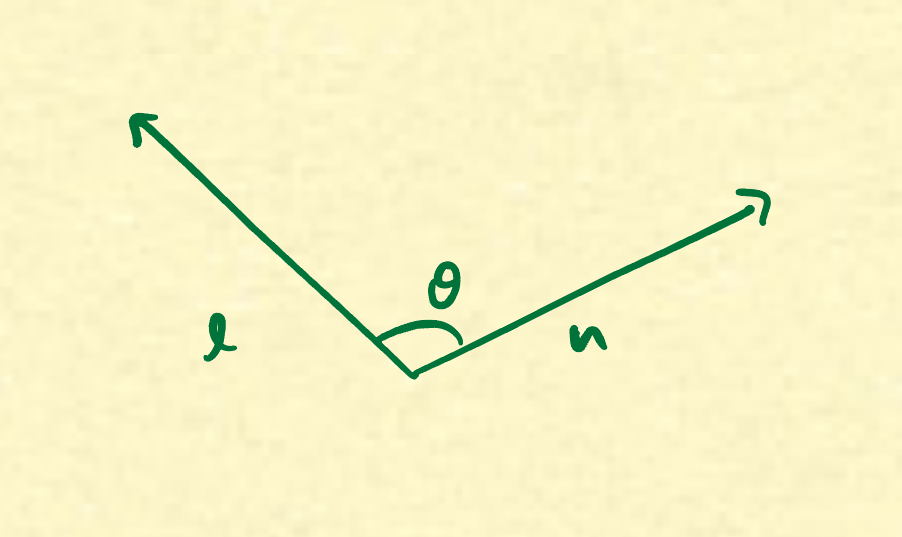
\includegraphics[width=0.3\textwidth,frame]{assets/ln.jpg}
	\hspace{0.2\textwidth}
	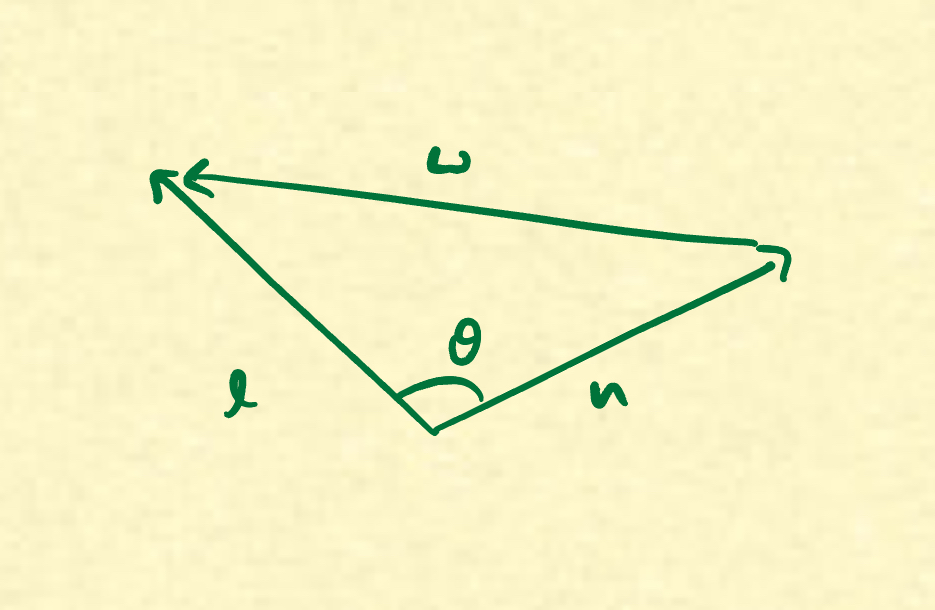
\includegraphics[width=0.2735\textwidth,frame]{assets/lnw.jpg}
\end{center}

The full Law of Cosines says that for any triangle with angles/sides labeled like so, we have $c^2 = a^2 + b^2 - 2ab \cos C$.
In our case, $a = |l|$, $b = |n|$, and $C = \theta$.
How can we compute the value of that third side length?

Vectors add by being placed tip to tail.
This means that the vector $\Delta$, which starts at $n$ and ends at $l$, is the thing that you can add to $n$ to get $l$: $l = n + \Delta => \Delta = l - n$.
So we have:

\begin{align*}
|l-n|^2 = |l|^2 + |n|^2 - 2 |l| |n| \cos \theta & \quad \text{substitute from generalized LoC} \\
|l-n|^2 = 2 - 2 \cos \theta & \quad \text{since we know } |l| = |n| = 1
\end{align*}

To help with this next part, I'm going to introduce some shorthand notation for an operation that we are performing.
The operation takes two vectors, performs a pairwise multiplication and sums the entries of the resulting vector.
The notation I will use to signify this is a $\cdot$ between two vectors: $a \cdot b$.

If we expand $|l - n|^2$ as $\sqrt{(l_x - n_x)^2 + (l_y - n_y)^2 + (l_z - n_z)^2} ^2$, our new notation comes in handy right away because we can rewrite that big expression as $\sqrt{(l - n) \cdot (l - n)}^2 = (l-n) \cdot (l - n)$.

\begin{align*}
(l - n) \cdot (l - n) = 2 - 2 \cos \theta & \quad \text{by using our new notation} \\
l \cdot l - l \cdot n - n \cdot l + n \cdot n = 2 - 2 \cos \theta & \quad \text{distribute (I'm cheating here for the sake of brevity)} \\
|l|^2 - 2 l \cdot n + |n|^2 = 2 - 2 \cos \theta & \quad \text{reversing our new notation} \\
1 - 2 l \cdot n + 1 = 2 - 2 \cos \theta & \quad \text{simplifying} \\
l \cdot n = \cos \theta & \quad \text{simplifying}
\end{align*}

Many of you have seen this result before.
For those of you who haven't, that ``dot'' symbol I introduced represents an operation commonly known as the dot product.
It is an exceedingly useful operation in mathematics and computer science, in large part because of the property that we just proved: that the dot product of two unit vectors is equal to the cosine of the angle between them.

\subsubsection{Takeaways}

I want you to take away a few things from this proof.

First: The Law of Cosines is true for all triangles -- even degenerate ones where the three points are co-linear or even identical!
So no matter what our two vectors are, we can compute the dot product $l \cdot n$ and it will always be $\cos \theta$!

Second: We didn't really assume that our vector had to be in 3-dimensions.
We only expanded our vector for x, y, and z but the same argument will hold for any dimension.

Third: This relationship also has a more general form.
We assumed that our two vectors had unit length, but we can make a slight tweak and then this result holds for any two vectors.
All we need to do is scale $\cos \theta$ by the lengths of the relevant vectors.
Given any two vectors $ a, b \in \mathbf{R}^n$: $a \cdot b = |a| |b| \cos \theta$.
It might be a fun exercise for you to build on this proof and show why that is the case.

Finally: I'd like you to recognize how surprising and elegant this result is.
I mean, it's crazy that combining two lists of numbers in this really simple way exactly matches $\cos \theta$.
Sometimes simple operations are really powerful.

\section{Final product}

So now back to our directional lighting.
From before, we want to light the terrain according to $\dfrac{1 + \cos \theta}{2}$ and we just proved that $\cos \theta = l \cdot n$.
Substituting that in, we have the final product, the light strength is $\dfrac{1 + l \cdot n}{2}$.
That's all it takes to produce the hillshade shown in these images.

\animation{Show a few examples.}

\section{Endnotes}

\subsection{Modified techniques}

Hillshading isn't just one thing.
It is actually a term for a family of effects that can be applied to a map.
There are a lot of variations out there.
Some examples include ambient lighting, exaggerating the normal vector, using multiple light sources, and playing around with colored lights.
You now have the mathematical framework that sits behind all of them.

\todo{Possibly mention Eduard Imhof.}

\subsection{Pseudoscopic Illusion}

In mapping, the light source for hillshade is typically placed in the northwest.
This is because most people recognize features better when the light is placed in the top left of an image, and because many maps use a north-up convention, that places the light source in the top left.

However, this can some backfire when a map with static hillshade is oriented with a south-up convention.
When that occurs, your brain might interpret everything backwards (valleys as ridges and ridges and valleys).
This is called a pseudoscopic illusion.

\animation{Show a south-up map light from the northwest and then fade in the same map (still south up) with a southeast (top left) light}.

\subsection{2D vs 3D}

I'd like to end the video by making one last comment on the simplicity of this effect: this is not a 3-dimensional map.
And I don't just mean that the screen you're viewing is 2-dimensional.
I mean that the actual model that I am rendering is 2D.

\animation{Pitch the camera}

Despite that, it is an incredibly effective method of conveying information about terrain.
I find that fascinating.

\animation{3D flythrough?}

\end{document}